\documentclass[12pt,letterpaper]{article}
\usepackage{graphicx,textcomp}
\usepackage{natbib}
\usepackage{setspace}
\usepackage{fullpage}
\usepackage{color}
\usepackage[reqno]{amsmath}
\usepackage{amsthm}
\usepackage{fancyvrb}
\usepackage{amssymb,enumerate}
\usepackage[all]{xy}
\usepackage{endnotes}
\usepackage{lscape}
\newtheorem{com}{Comment}
\usepackage{float}
\usepackage{hyperref}
\newtheorem{lem} {Lemma}
\newtheorem{prop}{Proposition}
\newtheorem{thm}{Theorem}
\newtheorem{defn}{Definition}
\newtheorem{cor}{Corollary}
\newtheorem{obs}{Observation}
\usepackage[compact]{titlesec}
\usepackage{dcolumn}
\usepackage{tikz}
\usetikzlibrary{arrows}
\usepackage{multirow}
\usepackage{subcaption}
\usepackage{xcolor}
\newcolumntype{.}{D{.}{.}{-1}}
\newcolumntype{d}[1]{D{.}{.}{#1}}
\definecolor{light-gray}{gray}{0.65}
\usepackage{url}
\usepackage{listings}
\usepackage{color}

\definecolor{codegreen}{rgb}{0,0.6,0}
\definecolor{codegray}{rgb}{0.5,0.5,0.5}
\definecolor{codepurple}{rgb}{0.58,0,0.82}
\definecolor{backcolour}{rgb}{0.95,0.95,0.92}

\lstdefinestyle{mystyle}{
	backgroundcolor=\color{backcolour},   
	commentstyle=\color{codegreen},
	keywordstyle=\color{magenta},
	numberstyle=\tiny\color{codegray},
	stringstyle=\color{codepurple},
	basicstyle=\footnotesize,
	breakatwhitespace=false,         
	breaklines=true,                 
	captionpos=b,                    
	keepspaces=true,                 
	numbers=left,                    
	numbersep=5pt,                  
	showspaces=false,                
	showstringspaces=false,
	showtabs=false,                  
	tabsize=2
}
\lstset{style=mystyle}
\newcommand{\Sref}[1]{Section~\ref{#1}}

\title{PS01 - My Answers (Quants 1)}
\date{09.10.2025}
\author{Sarah Magdihs}

\begin{document}
	\maketitle
	
	
	\section*{Question 1: Education }
	
	\textit{A school counselor was curious about the average of IQ of the students in her school and took a random sample of 25 students’ IQ scores. The following is the data set:.}\\
	
	\lstinputlisting[language=R, firstline=44, lastline=44]{PS01_answersSM.R}  
	
	\vspace{.25cm}
	
\begin{enumerate}
	\item Find a 90\% confidence interval for the average student IQ in the school.\\
	 
\noindent{\texttt{Answer:}} 
	
	\noindent {Let's start with the long version: As shown below, I calculated the sample size, the mean, the standard deviation and the standard error in order to then calculate the confidence interval "by hand". I use a t-value because n is smaller than 30.} 
	
		\vspace{.25cm}
	\noindent{\texttt{R Code:}} 
		\lstinputlisting[language=R, firstline=49, lastline=64]{PS01_answersSM.R}  
\begin{verbatim}
	[1]  93.95993 102.92007
	\end{verbatim}
	
	 \noindent {Thus, the 90 per cent confidence intervall is [93.96;102.92]. 
	 	This means that - with repeated sampling - the confidence interval contains the true parameter at least 90 per cent of the time. Hence, we can be 90 per cent confident that the interval [93.96;102.92] contains the population mean.} 
	 	
	 			\vspace{.25cm}
	\noindent {You can also cross-check this with a t-test:} 
		\vspace{.25cm}
		
		\noindent{\texttt{R Code:}} 
		\lstinputlisting[language=R, firstline=73, lastline=73]{PS01_answersSM.R}  

		\begin{verbatim}
			data:  y
			t = 37.593, df = 24, p-value < 2.2e-16
			alternative hypothesis: true mean is not equal to 0
			90 percent confidence interval:
			93.95993 102.92007
			sample estimates:
			mean of x 
			98.44 
		\end{verbatim}

	 \noindent {As we can see, the t-test also shows that the CI = [93.96;102.92].

 \noindent (Besides also doing other things). } 
			
			
		\item Next, the school counselor was curious  whether  the average student IQ in her school is higher than the average IQ score (100) among all the schools in the country.\\ 
	\noindent Using the same sample, conduct the appropriate hypothesis test with $\alpha=0.05$.
				\vspace{.5cm}
				
\noindent {Based on the information, this is a one-sided t-test, as the counselor wants to test whether the average student IQ at her school is **higher** than the mean of the population. 
	
	Thus, the hypotheses are as following:
	
	H0: mean is equal to or smaller than 100 

	Ha: mean bigger than 100
	
	Since alpha = 0.05, the confidence level is 95 per cent.} 
	\vspace{.25cm}
	
	\noindent{\texttt{Answer:}} 
	
	 \noindent {Let's start with the short version again: .} 

	\noindent{\texttt{R Code:}} 
		\lstinputlisting[language=R, firstline=97, lastline=97]{PS01_answersSM.R}  
		
		\begin{verbatim}
			data:  y
			t = -0.59574, df = 24, p-value = 0.7215
			alternative hypothesis: true mean is greater than 100
			95 percent confidence interval:
			93.95993      Inf
			sample estimates:
			mean of x 
			98.44 
		\end{verbatim}
		
		 \noindent {Based on this, the Null-Hypothesis cannot be rejected (p=0.7215, which is bigger than 0.05).
		 	Note that the p-value denotes the probability of seeing a value as extreme as this one (or higher) if the H0 was true.
		 
		 Moreover, we can see that the mean of the counselor's students is actually lower than the average for all students in the country (mean= 98.44). This is not only indicated by the 'mean of x' but also by the negative t-value.} 
			\vspace{.25cm}
		
			 \noindent {Furthermore, as discussed in the lecture, we can technically also do this step by step ourselves.} 
		
			\noindent{\texttt{R Code:}} 
			\lstinputlisting[language=R, firstline=113, lastline=123]{PS01_answersSM.R}  
		
			\begin{verbatim}
			      Mean   StdError          t         df    p_value 
			98.4400000  2.6185747 -0.5957439 24.0000000  0.7215383
		\end{verbatim}
		
\end{enumerate}

	\section*{Question 2: Political Economy }
	
	\textit{Researchers are curious about what affects the amount of money communities spend on addressing homelessness. The following variables constitute our data set about social welfare expenditures in the USA.}\\
			\vspace{.5cm}
			
\begin{tabular}{r|l}
	\texttt{State} &\emph{50 states in US} \\
	\texttt{Y} & \emph{per capita expenditure on shelters/housing assistance in state}\\
	\texttt{X1} &\emph{per capita personal income in state} \\
	\texttt{X2} &  \emph{Number of residents per 100,000 that are "financially insecure" in state}\\
	\texttt{X3} &  \emph{Number of people per thousand residing in urban areas in state} \\
	\texttt{Region} &  \emph{1=Northeast, 2= North Central, 3= South, 4=West} \\
\end{tabular}

			\vspace{.5cm}
			\noindent {Explore the expenditure data set and import data into \texttt{R}.} 
			\vspace{.5cm}
		
		\vspace{.5cm}
			\noindent{\texttt{Okay, so let's load and inspect our data first:}} 
		\vspace{.25cm}
		
	\noindent{\texttt{R Code:}} 
\lstinputlisting[language=R, firstline=141, lastline=143]{PS01_answersSM.R}  
			
		\begin{verbatim}
				> head(expenditure)
				STATE  Y   X1  X2  X3 Region
				1    ME 61 1704 388 399      1
				2    NH 68 1885 272 598      1
				3    VT 72 1745 397 370      1
				4    MA 72 2394 458 868      1
				5    RI 62 1966 157 899      1
				6    CT 91 2817 162 690      1
				> str(expenditure)
				'data.frame':	50 obs. of  6 variables:
				$ STATE : chr  "ME" "NH" "VT" "MA" ...
				$ Y     : int  61 68 72 72 62 91 120 99 70 82 ...
				$ X1    : int  1704 1885 1745 2394 1966 2817 2685 2521 2127 2184 ...
				$ X2    : int  388 272 397 458 157 162 494 153 152 187 ...
				$ X3    : int  399 598 370 868 899 690 728 826 656 674 ...
				$ Region: int  1 1 1 1 1 1 1 1 1 2 ...
		\end{verbatim}
					\vspace{.5cm}
\begin{enumerate}
	\item Please plot the relationships among Y, X1, X2, and X3 ? What are the correlations among them (you just need to describe the graph and the relationships among them)?\\

\noindent{\texttt{Answer:}} 

\noindent {In order to plot the relationships between these variables, I will use a scatterplot. However, I don't want to plot each combination individually, as that is really tedious. Instead, let's use the pairs command.} 
					\vspace{.5cm}
					
 	\noindent{\texttt{R Code:}} 
 \lstinputlisting[language=R, firstline=151, lastline=154]{PS01_answersSM.R} 

\begin{center}
	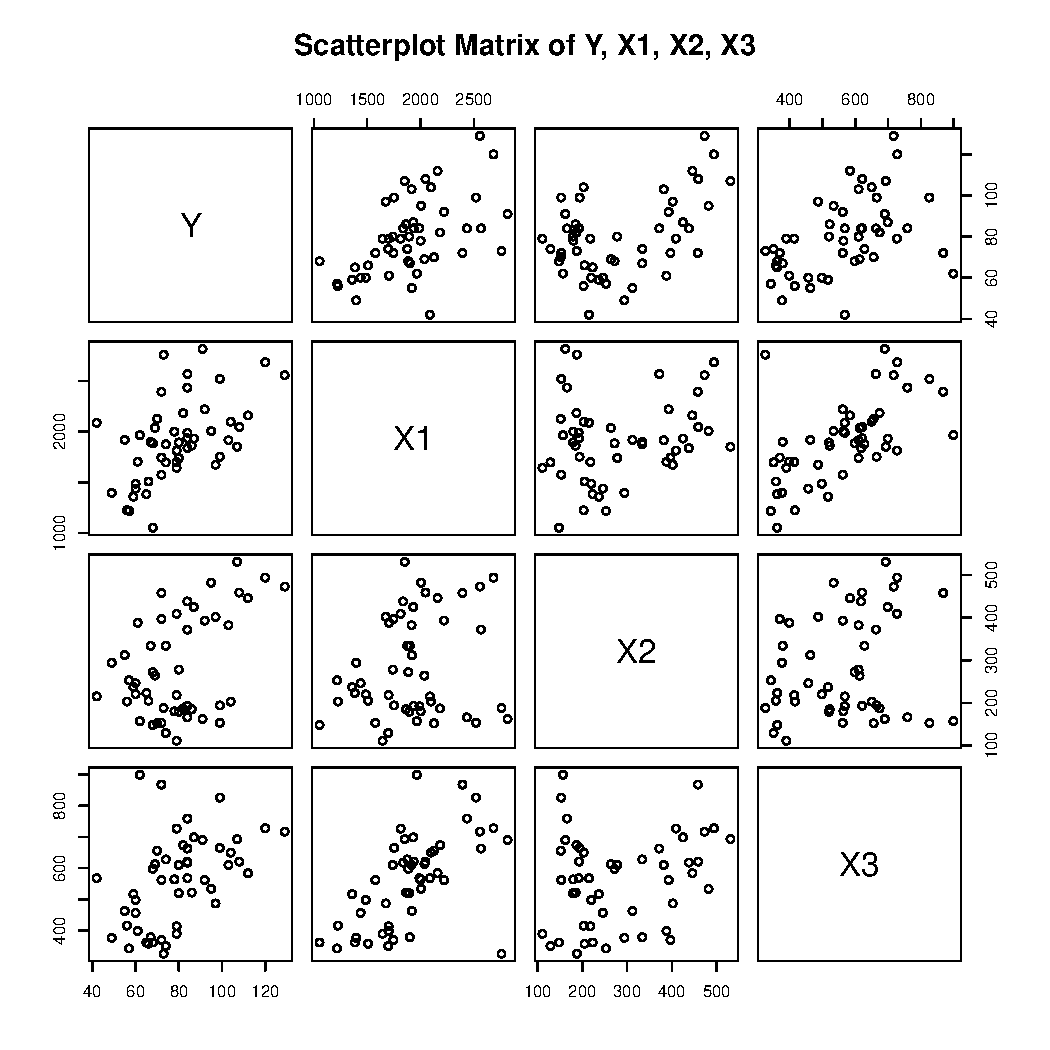
\includegraphics[width=0.5\textwidth]{Plot_Matrix.pdf}
\end{center}

\noindent {So, that covers the plotting. To assess the relationships, looking at data is important, but sometimes correlations (or assosciations) can be hard to gauge visually. So let's use a correlation matrix before we move to the interpretation.} 

\noindent{\texttt{R Code:}} 
\lstinputlisting[language=R, firstline=157, lastline=160]{PS01_answersSM.R} 

	\begin{verbatim}
	      Y   X1   X2   X3
	Y  1.00 0.53 0.45 0.46
	X1 0.53 1.00 0.21 0.60
	X2 0.45 0.21 1.00 0.22
	X3 0.46 0.60 0.22 1.00
\end{verbatim}


\noindent{\texttt{Now for the description/interpretation:}} 

\noindent {Generally, the created plot includes all possible correlation plot between the four variables. The diagonal only shows the variable names, since each variable obviously perfectly correlates with itself. The correlations above and below the diagonal are mirrored (since it shows, for example, the correlation of Y and X1, as well as X1 and Y). So, I will focus on the plots below the diagonal. } 

\noindent {There seems to be a moderate positive correlation between Y and X1; Y and X2; Y and X3. Thus, based on the plots and the correlation coefficients, states that have a higher per capita personal income/more financially insecure residence/a higher urban population density, tend to spend more money on shelters/housing assistance. } 

\noindent {Moreover, X1 and X3 have an r = 0.6, which means that there could be collinearity issues when a regression model uses both variables as predictors.} 

\noindent {Lastly, X1 and X2 are only weakly correlated (but seem somewhat linear).X2 and X3 have a low correlation coefficient (r=0.22) which indicates that there is at best a weak linear correlation. This also makes sense when looking at the graphs: The scatterplot of X2 and X3 looks like their assosciation may be better described by a quadratic function. } 


	\item Please plot the relationship between Y and Region? On average, which region has the highest per capita expenditure on housing assistance?.\\ 

\noindent{\texttt{Answer:}} 

\noindent {To look at the relationship between Expenditure and Region, we can use boxplots. However, when I inspected the data, it showed that Region is an integer - which will be an issue for a boxplot. So let's make it a factor. } 


\noindent{\texttt{R Code:}} 
\lstinputlisting[language=R, firstline=172, lastline=178]{PS01_answersSM.R} 

\noindent {Now, we can make boxplots:} 

\noindent{\texttt{R Code:}} 
\lstinputlisting[language=R, firstline=182, lastline=188]{PS01_answersSM.R} 

\begin{center}
	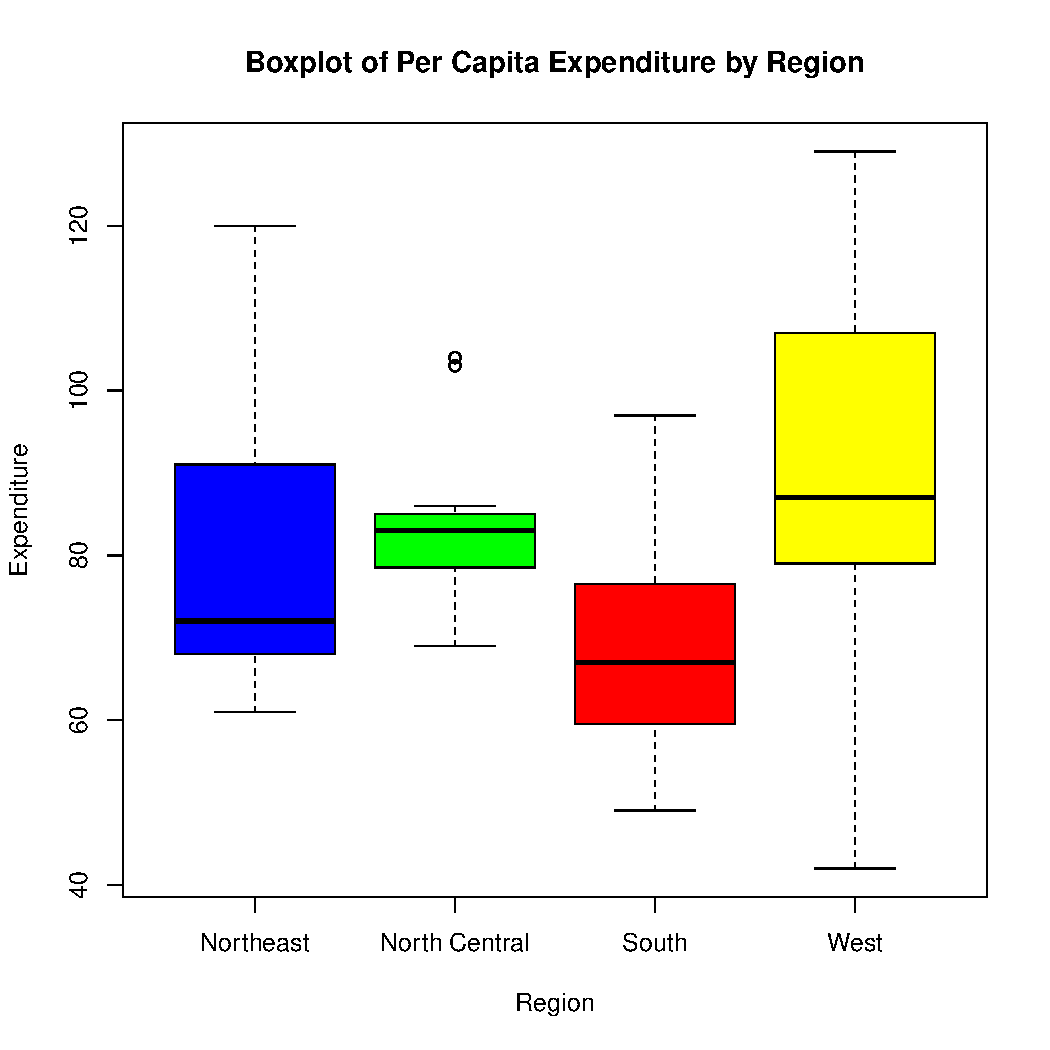
\includegraphics[width=0.5\textwidth]{boxplot_Y_Region.pdf}
\end{center}


\noindent {However, the second question is about the average, but boxplots give us the median. 
	In this case, I think the difference should not be drastic. But since averages our outlier sensitive, let's make sure it actually doesn't make a difference.} 

\noindent{\texttt{R Code:}} 
\lstinputlisting[language=R, firstline=193, lastline=205]{PS01_answersSM.R} 

\begin{center}
	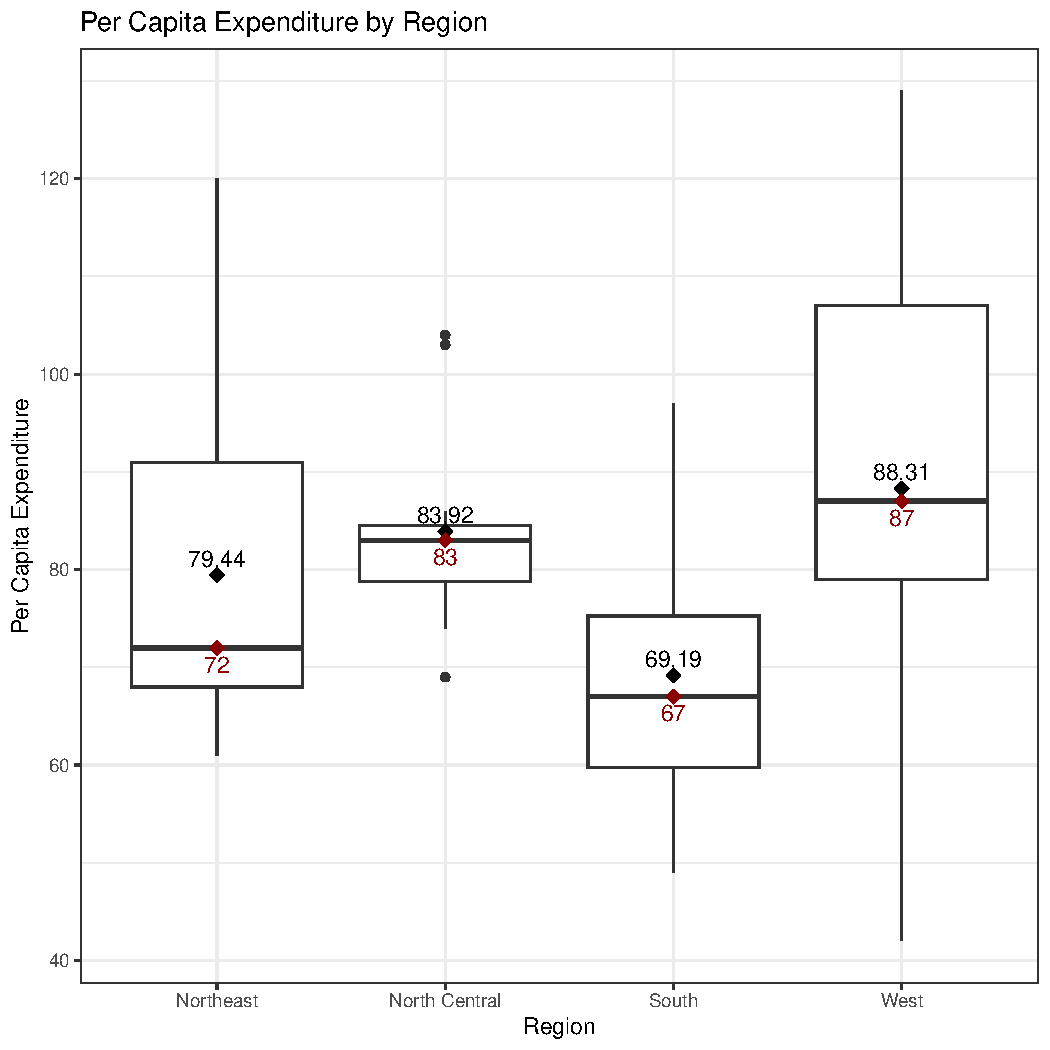
\includegraphics[width=0.5\textwidth]{boxplot_with_average.pdf}
\end{center}

	\noindent {As expected, in this case it doesn't really make a difference regarding the interpretation (despite the mean and median slightly diverging).
	
	Here, we see that on average states in the Region "West" have the highest per capita expenditure on shelters/housing assistance. } 

	\item Please plot the relationship between Y and X1 ? Describe this graph and the relationship. Reproduce the above graph including one more variable Region and display different regions with different types of symbols and colors..\\ 
	
	\noindent{\texttt{Answer:}} 
	
	\noindent {Let's start with the simple plot: } 
	
\noindent{\texttt{R Code:}} 
\lstinputlisting[language=R, firstline=214, lastline=223]{PS01_answersSM.R} 

\begin{center}
	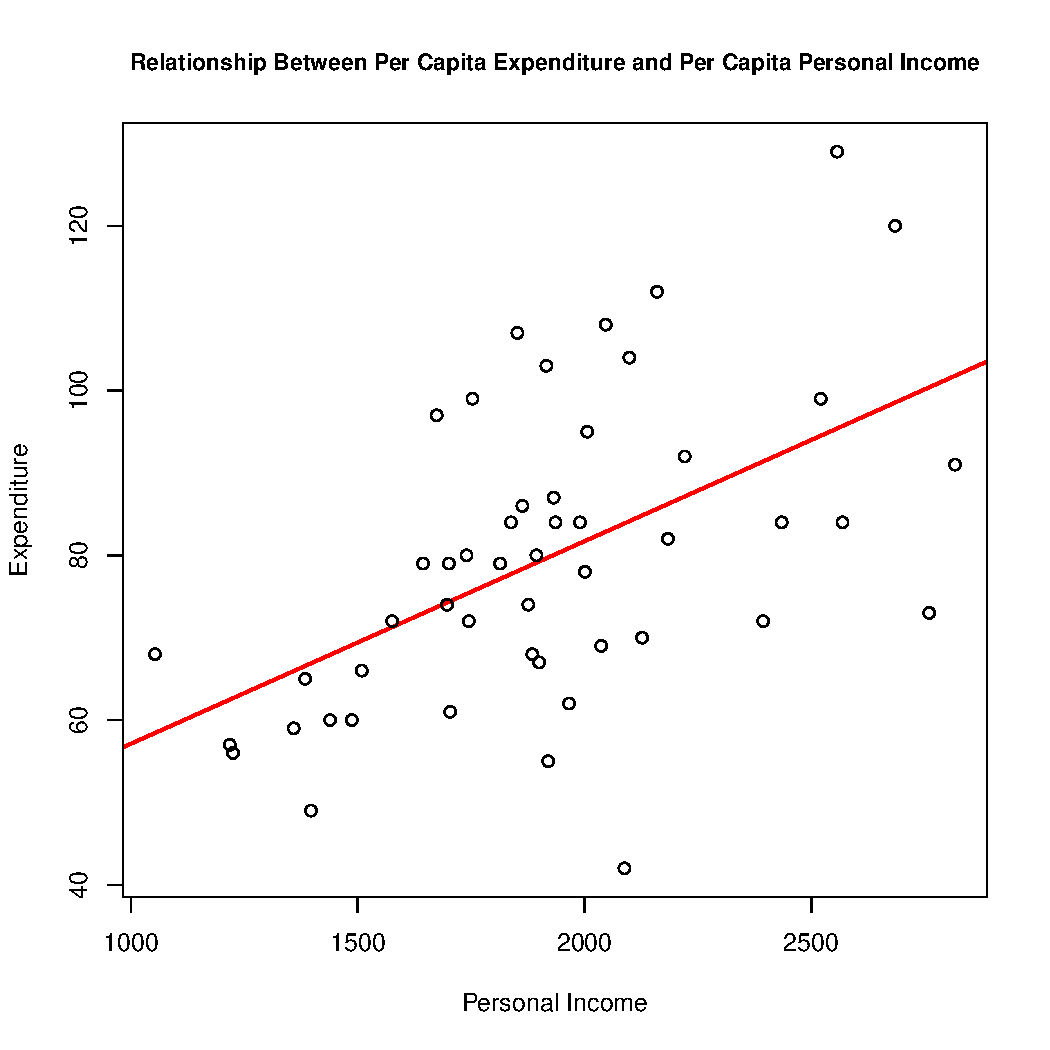
\includegraphics[width=0.5\textwidth]{Task2_3_basic.pdf}
\end{center}


	\noindent {As already mentioned during the discussion of the scatterplots and potential correlations, we can see here that there is some kind of positive linear assosciation between per capita personal income and per capita expenditure on shelters/housing assistance. More concretely, states that have higher per capita personal income tend to spend more money on shelters/housing assistance.
	
	The added regression line helps visualise this relationship more effectively.} 
	
						\vspace{.5cm}

	\noindent {Lastly, let's reproduce the above graph including one more variable Region and display different regions with different types of symbols and colors.} 

\noindent{\texttt{R Code:}} 
\lstinputlisting[language=R, firstline=230, lastline=253]{PS01_answersSM.R} 


\begin{center}
	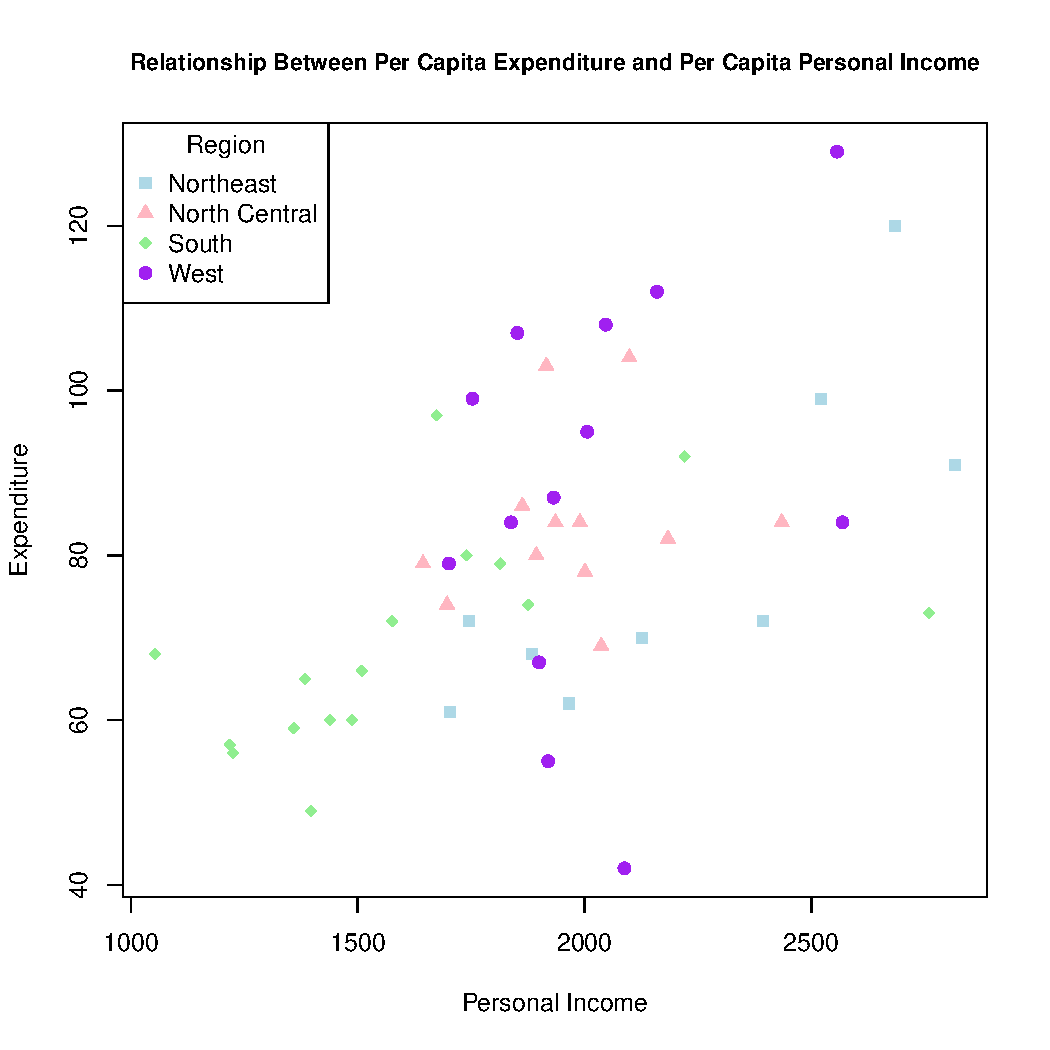
\includegraphics[width=0.5\textwidth]{Task2_3_with_Colours_and_Symbols.pdf}
\end{center}

\begin{enumerate}

		
\end{document}